% Options for packages loaded elsewhere
\PassOptionsToPackage{unicode}{hyperref}
\PassOptionsToPackage{hyphens}{url}
%
\documentclass[
  12pt,
]{article}
\usepackage{amsmath,amssymb}
\usepackage{iftex}
\ifPDFTeX
  \usepackage[T1]{fontenc}
  \usepackage[utf8]{inputenc}
  \usepackage{textcomp} % provide euro and other symbols
\else % if luatex or xetex
  \usepackage{unicode-math} % this also loads fontspec
  \defaultfontfeatures{Scale=MatchLowercase}
  \defaultfontfeatures[\rmfamily]{Ligatures=TeX,Scale=1}
\fi
\usepackage{lmodern}
\ifPDFTeX\else
  % xetex/luatex font selection
\fi
% Use upquote if available, for straight quotes in verbatim environments
\IfFileExists{upquote.sty}{\usepackage{upquote}}{}
\IfFileExists{microtype.sty}{% use microtype if available
  \usepackage[]{microtype}
  \UseMicrotypeSet[protrusion]{basicmath} % disable protrusion for tt fonts
}{}
\makeatletter
\@ifundefined{KOMAClassName}{% if non-KOMA class
  \IfFileExists{parskip.sty}{%
    \usepackage{parskip}
  }{% else
    \setlength{\parindent}{0pt}
    \setlength{\parskip}{6pt plus 2pt minus 1pt}}
}{% if KOMA class
  \KOMAoptions{parskip=half}}
\makeatother
\usepackage{xcolor}
\usepackage[margin=1in]{geometry}
\usepackage{longtable,booktabs,array}
\usepackage{calc} % for calculating minipage widths
% Correct order of tables after \paragraph or \subparagraph
\usepackage{etoolbox}
\makeatletter
\patchcmd\longtable{\par}{\if@noskipsec\mbox{}\fi\par}{}{}
\makeatother
% Allow footnotes in longtable head/foot
\IfFileExists{footnotehyper.sty}{\usepackage{footnotehyper}}{\usepackage{footnote}}
\makesavenoteenv{longtable}
\usepackage{graphicx}
\makeatletter
\def\maxwidth{\ifdim\Gin@nat@width>\linewidth\linewidth\else\Gin@nat@width\fi}
\def\maxheight{\ifdim\Gin@nat@height>\textheight\textheight\else\Gin@nat@height\fi}
\makeatother
% Scale images if necessary, so that they will not overflow the page
% margins by default, and it is still possible to overwrite the defaults
% using explicit options in \includegraphics[width, height, ...]{}
\setkeys{Gin}{width=\maxwidth,height=\maxheight,keepaspectratio}
% Set default figure placement to htbp
\makeatletter
\def\fps@figure{htbp}
\makeatother
\setlength{\emergencystretch}{3em} % prevent overfull lines
\providecommand{\tightlist}{%
  \setlength{\itemsep}{0pt}\setlength{\parskip}{0pt}}
\setcounter{secnumdepth}{5}
\newlength{\cslhangindent}
\setlength{\cslhangindent}{1.5em}
\newlength{\csllabelwidth}
\setlength{\csllabelwidth}{3em}
\newlength{\cslentryspacingunit} % times entry-spacing
\setlength{\cslentryspacingunit}{\parskip}
\newenvironment{CSLReferences}[2] % #1 hanging-ident, #2 entry spacing
 {% don't indent paragraphs
  \setlength{\parindent}{0pt}
  % turn on hanging indent if param 1 is 1
  \ifodd #1
  \let\oldpar\par
  \def\par{\hangindent=\cslhangindent\oldpar}
  \fi
  % set entry spacing
  \setlength{\parskip}{#2\cslentryspacingunit}
 }%
 {}
\usepackage{calc}
\newcommand{\CSLBlock}[1]{#1\hfill\break}
\newcommand{\CSLLeftMargin}[1]{\parbox[t]{\csllabelwidth}{#1}}
\newcommand{\CSLRightInline}[1]{\parbox[t]{\linewidth - \csllabelwidth}{#1}\break}
\newcommand{\CSLIndent}[1]{\hspace{\cslhangindent}#1}
\usepackage{titling}
\pretitle{\begin{center} 
\includegraphics[width=2in,height=2in]{cerrilogo.jpg}\LARGE\\}
\posttitle{\end{center}}
\ifLuaTeX
  \usepackage{selnolig}  % disable illegal ligatures
\fi
\IfFileExists{bookmark.sty}{\usepackage{bookmark}}{\usepackage{hyperref}}
\IfFileExists{xurl.sty}{\usepackage{xurl}}{} % add URL line breaks if available
\urlstyle{same}
\hypersetup{
  pdftitle={Winipakw Climate Change, Contaminants and Blue Carbon Ecosystems Community-based Monitoring Project: Progress Report},
  pdfauthor={Dante Torio, Nicholas Chakapash, Preston Sam, Clara Rogers},
  hidelinks,
  pdfcreator={LaTeX via pandoc}}

\title{Winipakw Climate Change, Contaminants and Blue Carbon Ecosystems
Community-based Monitoring Project: Progress Report}
\usepackage{etoolbox}
\makeatletter
\providecommand{\subtitle}[1]{% add subtitle to \maketitle
  \apptocmd{\@title}{\par {\large #1 \par}}{}{}
}
\makeatother
\subtitle{Chisasibi Eeyou Resource and Research Institute}
\author{Dante Torio, Nicholas Chakapash, Preston Sam, Clara Rogers}
\date{22 May, 2024}

\begin{document}
\maketitle

{
\setcounter{tocdepth}{2}
\tableofcontents
}
\newpage

\hypertarget{background}{%
\section{Background}\label{background}}

This project aims to build scientific capacity in Chisasibi by
monitoring blue carbon ecosystems using environmental indicators
stemming from Cree Traditional Ecological Knowledge (TEK) and
environmental sciences. This project is one element of a longer-term
initiative to develop an integrated, Indigenous-led, landscape-level
conservation strategy across James Bay. In James Bay, blue carbon
habitats are essential for their global contribution to climate change
mitigation and their close link to sustaining the indigenous Cree way of
life as crucial habitats for fish and migratory waterfowl. We focus on
monitoring key blue carbon ecosystem indicators and assessing current
and emerging threats to these systems and their potential impacts on
Cree's traditional livelihoods. Through this project, we wish to build a
framework for participatory environmental monitoring in Chisasibi that
can be scaled up in other communities and contribute to conserving the
blue carbon ecosystems in eastern James Bay.

\hypertarget{objective}{%
\section{Objective}\label{objective}}

This project aims to initiate a long-term monitoring program to support
community-driven decision-making on environmental conservation locally
and across James Bay. Our approach is to monitor a suite of biophysical
and climate change indicators in strategic blue carbon ecosystems using
Cree TEK and scientific methods. Assessments will understand the
cumulative impacts and emerging threats to these ecosystems. Monitoring
activities will concentrate on the north of La Grande river. Using
monitoring data, we hope to gain the necessary depth and breadth of
knowledge to understand blue carbon ecosystems' current and future
state, ecosystem services, and impacts on traditional practices through
this strategy.

\hypertarget{methods}{%
\section{Methods}\label{methods}}

We visited several sites (see Figure \ref{fig:sites}) during the summer
of 2021, 2022, and 2023. We collected the following baseline data on
eelgrass habitats using a suite of environmental monitoring methods.

\begin{verbatim}
## Warning: package 'knitr' was built under R version 4.2.3
\end{verbatim}

\begin{figure}

{\centering 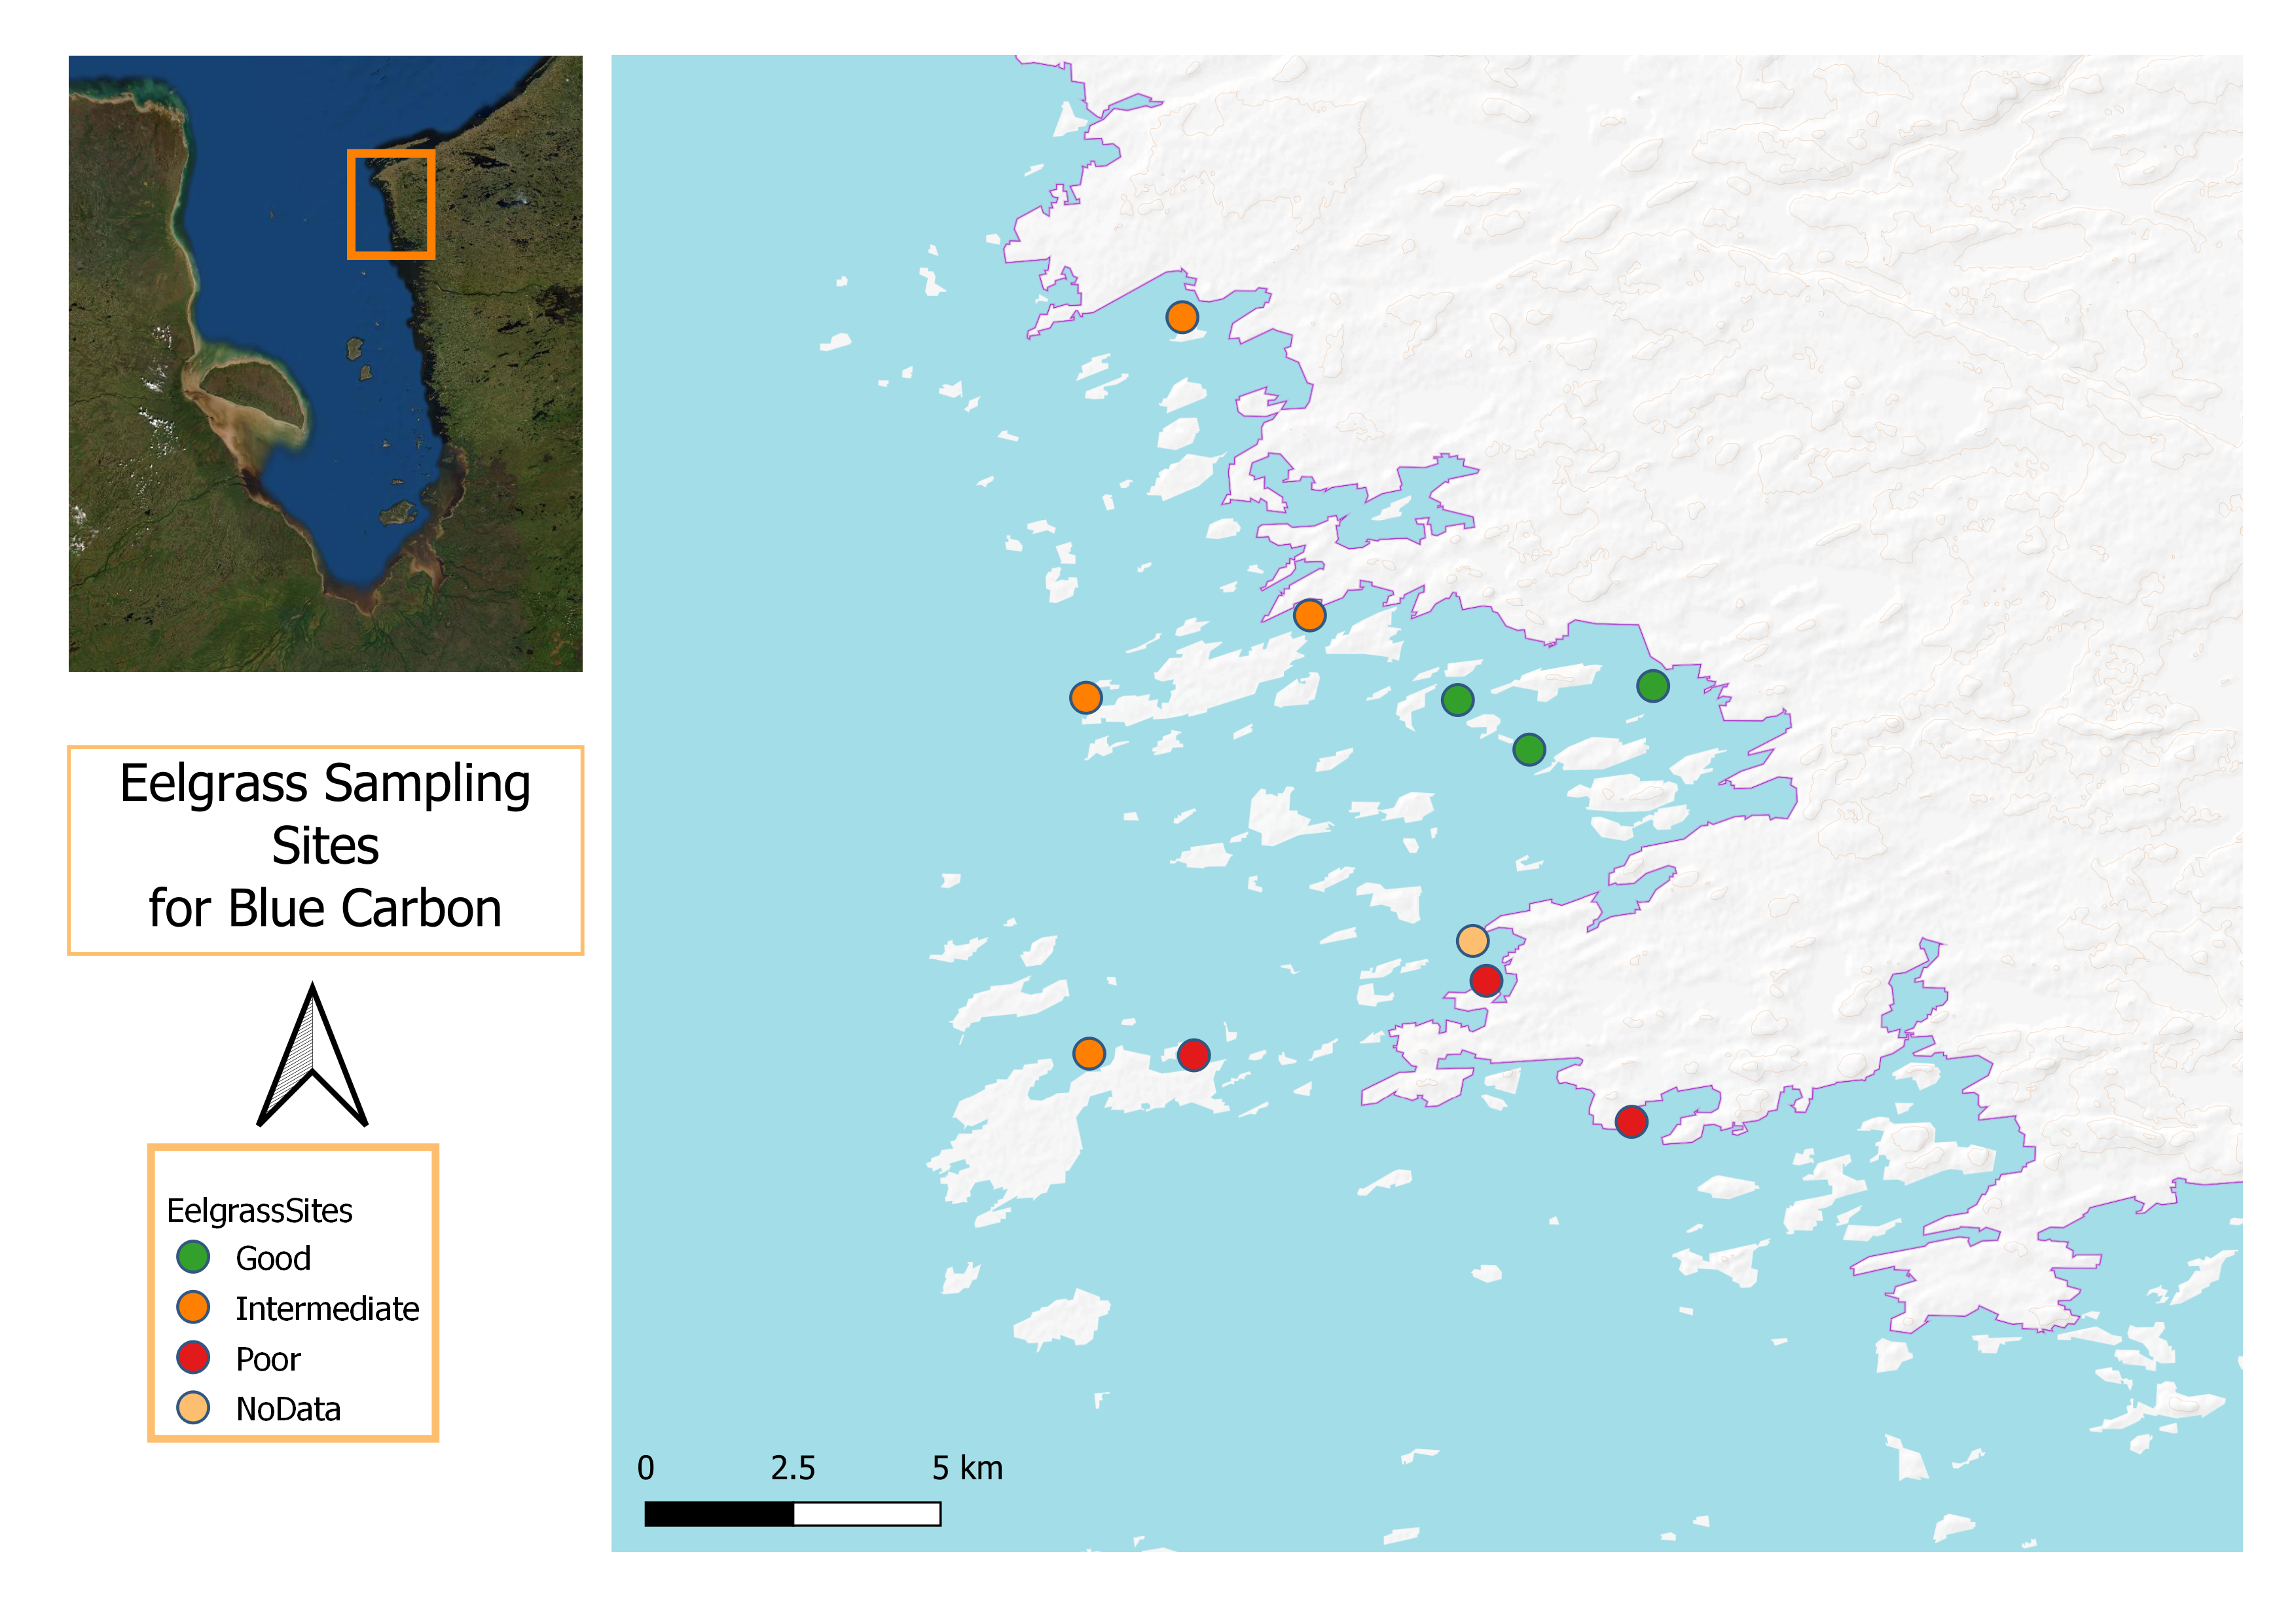
\includegraphics[width=1\linewidth]{BlueCarbonSites} 

}

\caption{Eelgrass ecosystem sampling locations}\label{fig:sites}
\end{figure}

\begin{itemize}
\tightlist
\item
  Sediment cores: Coring techniques followed a protocol by Howard and
  colleagues (2014).
\item
  Historical and current distribution derived from satellite remove
  sensing and ground survey
\item
  Collection and measurement of plant samples
\item
  Water quality indicators using multi-parameter instruments, moored
  sensor and CTDs
\item
  Presence or absence of potentially harmful algal blooms are determined
  using underwater camera and manual scooping.
\end{itemize}

We sent two sediment cores for analysis to the GEOTOP lab at the
University of Quebec in Montreal to measure organic carbon determine the
age of each section of the sediments using Lead assay(Pb210) techniques.
The data were analyzed at CERRI for age and sediment accretion rates
using Bayesian statistics (Aquino-López et al. 2018). Using the results
of the analyses we answered the following research questions:

\begin{enumerate}
\def\labelenumi{\arabic{enumi}.}
\tightlist
\item
  How much organic carbon (C) is James Bay blue carbon ecosystems
  accumulating per unit area per year?
\item
  What are the threats to blue carbon ecosystems, and how do these
  threats affect the sequestration rate of blue carbon in James Bay and
  their traditional ecosystem services?
\item
  What is the state of James Bay eelgrass and other coastal ecosystems
  as blue carbon sinks/sources?
\item
  How does climate change impact blue carbon accumulation in James Bay?
\item
  What management actions best maintain and promote carbon sequestration
  and traditional use of blue carbon ecosystems in James Bay?
\end{enumerate}

\hypertarget{general-project-accomplishments}{%
\section{General Project
Accomplishments}\label{general-project-accomplishments}}

\hypertarget{procurement-of-laboratory-equipment}{%
\subsection{Procurement of laboratory
equipment}\label{procurement-of-laboratory-equipment}}

\textbf{Percent accomplishment: 100}

Despite delays in procurement and delivery, the project acquired needed
scientific and field equipment and successfully carried out fieldwork.
All the equipment and consumables needed for water quality monitoring
have been delivered. Purchase of additional equipment is ongoing.

\hypertarget{sampling-program}{%
\subsection{Sampling program}\label{sampling-program}}

\textbf{Percent accomplishment: 100}

The trapline tallymen provided the knowledge that guided site selection.
These sites are precise and have a long history of resource use and they
also represent areas where land users have observed environmental
changes throughout the years. Last fall, we finally collected sediment
cores from 2 target sites, one with thriving eelgrass and one from
marginal eelgrass beds.

\hypertarget{analyses-of-core-samples}{%
\subsection{Analyses of core samples}\label{analyses-of-core-samples}}

\textbf{Percent accomplishment: 100 }

Since istotopic and organic content analyses are not possible with the
current setup at CERRI, two cores were sent out to the GEOTOP lab at the
University of Quebec in Montreal. The results has been received and
interpretation of the data are finished.

\hypertarget{hiring-and-training-of-local-youth}{%
\subsection{Hiring and training of local
youth}\label{hiring-and-training-of-local-youth}}

\textbf{Percent accomplishment: 100 }

The funding contributed to the partial salaries of two local youth
co-researchers. These co-researchers were involved in all the fieldwork
and were trained to conduct core sampling and preparation of core
sections. They received training in using a universal coring device,
core extrusion, and core sectioning in the field.

\hypertarget{community-presentation}{%
\subsection{Community presentation}\label{community-presentation}}

\textbf{Percent accomplishment: 90 }

We made two presentations to the CERRI board about the project and one
presentation to the general community assembly. Community members were
learning blue carbon and climate change concepts. The community were
interested in exploring the synergy between enhancing the blue carbon
ecosystem to make them more productive as a carbon sink and waterfowl
habitats. They also wanted to know more about algae and cyanobacteria
and how it affects traditional resources like fisheries. Another
community presentation is planned in July to report back to the
community the results of the research.

\newpage

\hypertarget{research-results}{%
\section{Research results}\label{research-results}}

\hypertarget{general-eelgrass-state-and-ecology}{%
\subsection{General eelgrass state and
ecology}\label{general-eelgrass-state-and-ecology}}

Eelgrass beds at the two coring sites are marginally different. Eelgrass
plants on the first site (Core Site 04) were healthier and cleaner, and
had longer leaves. On the contrary, the second sampling location has
marginal to no eelgrass growth (Core site 01). Also, the second eelgrass
site had enourmous mats of microalgae and cyanobacteria (Figure
\ref{fig:bacteria} ). We identified these species belonging to the
family \emph{Oscillatoriaceae}, probably \emph{Oscillatoria spp} or
\emph{Lyngbya confervoides} previously recorded by Mathieson and
company(2010).

\begin{figure}

{\centering 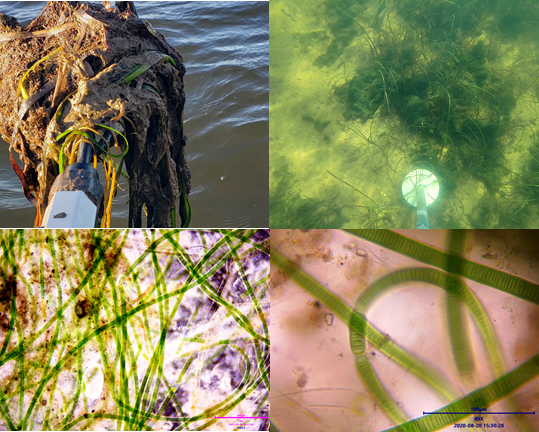
\includegraphics[width=1\linewidth]{CyanoBacteria} 

}

\caption{Mats and microscopic images of filamentous cyanobacteria}\label{fig:bacteria}
\end{figure}

\hypertarget{sediment-core-characteristics}{%
\subsection{Sediment core
characteristics}\label{sediment-core-characteristics}}

The sediment cores varied in length and substrate characteristics
(Figure \ref{fig:cores}). The site with eelgrass had the deepest
sediment at 96 cm while the marginal eelgrass site had about 65 cm. In
addition, the site with eelgrass is more silty and clayey while the
other site had more sand.

\begin{figure}

{\centering 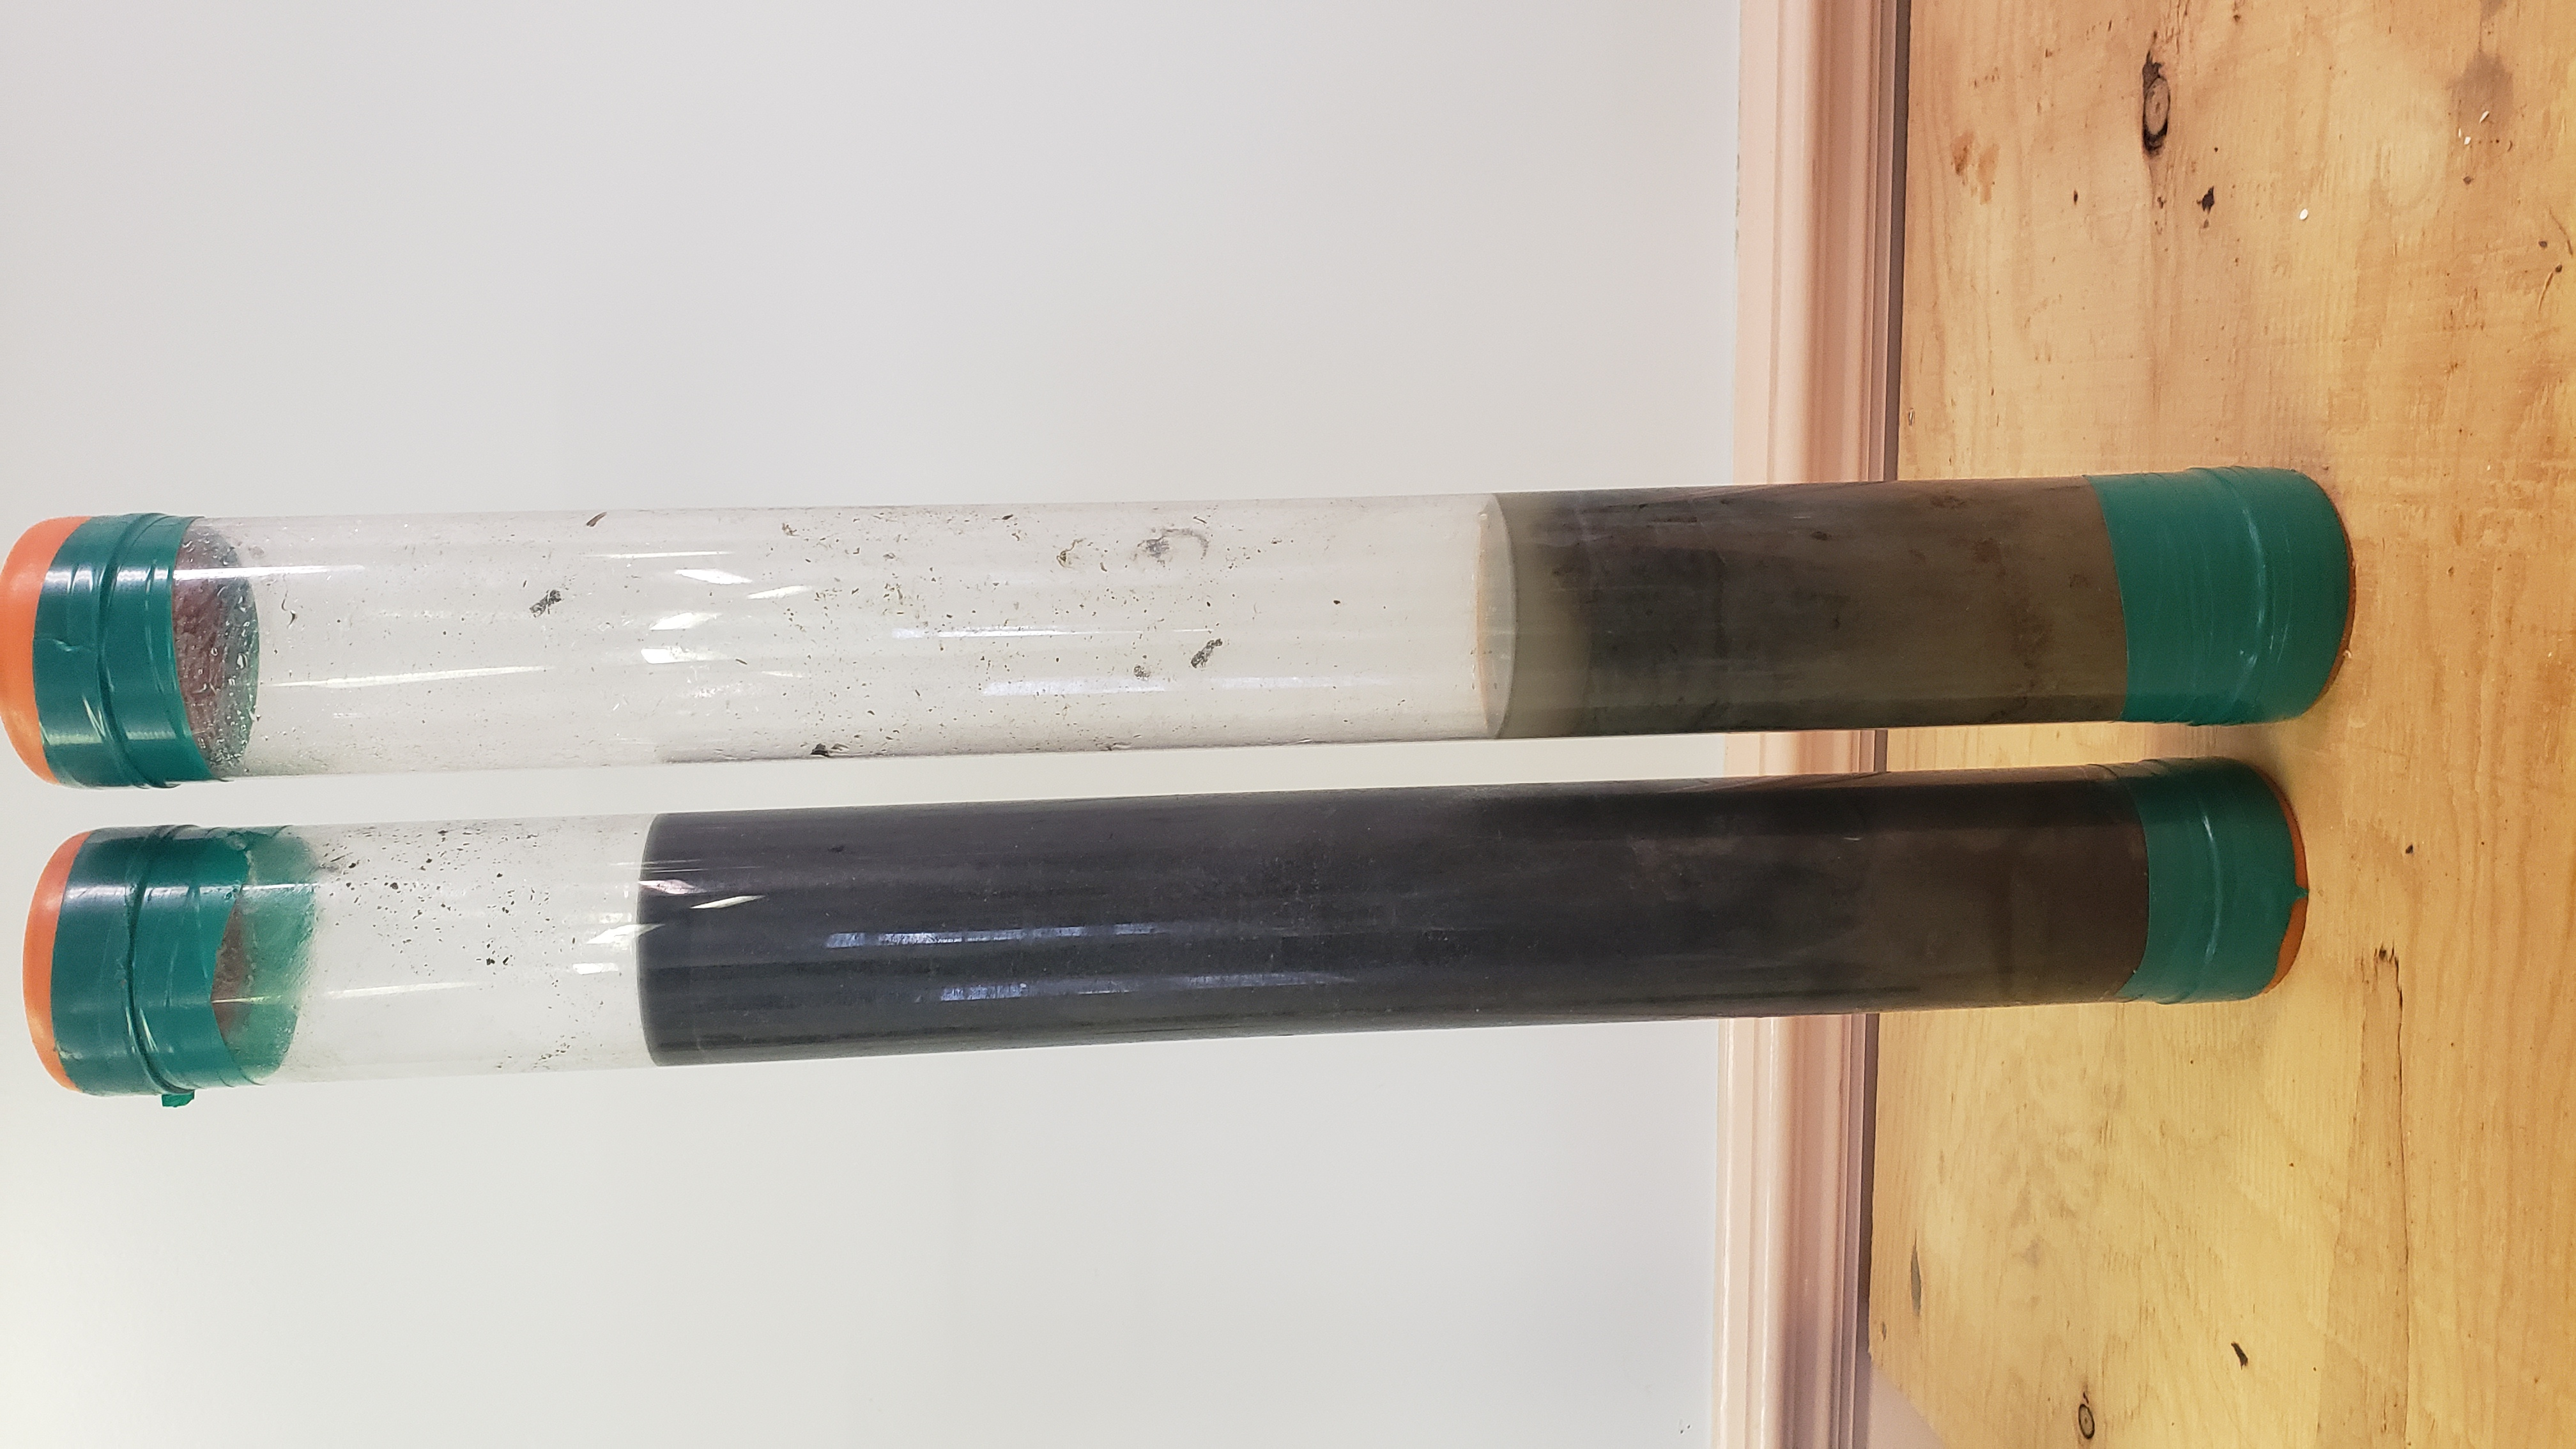
\includegraphics[width=0.5\linewidth,angle=-90]{sedcores} 

}

\caption{Eelgrass sediment cores}\label{fig:cores}
\end{figure}

\hypertarget{isotope-analyses}{%
\subsubsection{Isotope Analyses}\label{isotope-analyses}}

Stable isotope analyses provide valuable insights into the nature of
James Bay eelgrass sediments. The results are expressed in delta
notation (\(\delta\)) measures the ratios of stable isotopes of
carbon(13C/12C) and nitrogen(15N/14N) in samples. Results expressed as
part per thousand (ppt) deviation from a standard material. \(\delta\)
13C values provides information of the carbon sources in the sediment
while \(\delta\) 15N values values provide information about the
nitrogen sources and cycling in the ecosystem. In marine environments,
\(\delta\) 15N values can vary widely, influenced by sources of nitrogen
(like upwelling, nitrogen fixation, or anthropogenic inputs) and
processes like denitrification.

The \(\delta\) 13C ranges are typicall between -300‰ to +50‰. More
negative values indicate a dominance of terrestrial influence (tress and
shrubs-C3 plants), while less negative values suggest marine sources (C4
plants). Typical \(\delta\) 13C values of seagrass is around -11‰
closely resembling C4 species. C3 and c4 plants in terrestrial
environments have \(\delta\) 13C values around -28‰ to -14‰,
respectively (Touchette and Burkholder 2000).

The \(\delta\) 13C results from the core sample with eelgrass (C04)
ranges from -14.7‰ to -24.91‰ while the core with marginal eelgrass
(C01) ranges from -15.97‰ to -20.58‰. The more negative values in lower
end of core C04 values indicate significant incorporation or mixing of
terrestrial organic matter, which is typically more 13C-depleted
compared to marine organic matter while the range of values in Core 01
suggests a predominance of marine organic carbon with a possible minor
influence from terrestrial sources(Canuel et al., 1997).

On the other hand, the \(\delta\) 15N values in core C01 (marginal
eelgrass) range from +2.00‰ to +5.71‰ and the core with healthy eelgrass
(C04) had \(\delta\) 15N values between 1.79‰ and 4.44‰both suggest that
marine primary production and early consumer interactions dominate
(eelgrass and phytoplankton) as sources of nitrogen with little
influence from denitrification or terrestrial inputs.

\hypertarget{percent-organic-carbon}{%
\subsubsection{Percent Organic Carbon}\label{percent-organic-carbon}}

The core from marginal eelgrass has more organic carbon than the core
from healthy looking eelgrass see Table 1.

\begin{longtable}[]{@{}
  >{\raggedright\arraybackslash}p{(\columnwidth - 16\tabcolsep) * \real{0.1884}}
  >{\raggedleft\arraybackslash}p{(\columnwidth - 16\tabcolsep) * \real{0.0870}}
  >{\raggedleft\arraybackslash}p{(\columnwidth - 16\tabcolsep) * \real{0.1014}}
  >{\raggedleft\arraybackslash}p{(\columnwidth - 16\tabcolsep) * \real{0.1449}}
  >{\raggedleft\arraybackslash}p{(\columnwidth - 16\tabcolsep) * \real{0.0725}}
  >{\raggedleft\arraybackslash}p{(\columnwidth - 16\tabcolsep) * \real{0.1159}}
  >{\raggedleft\arraybackslash}p{(\columnwidth - 16\tabcolsep) * \real{0.1014}}
  >{\raggedleft\arraybackslash}p{(\columnwidth - 16\tabcolsep) * \real{0.1159}}
  >{\raggedleft\arraybackslash}p{(\columnwidth - 16\tabcolsep) * \real{0.0725}}@{}}
\caption{Summary Statistics of Percent Organic Carbon}\tabularnewline
\toprule\noalign{}
\begin{minipage}[b]{\linewidth}\raggedright
SITEID
\end{minipage} & \begin{minipage}[b]{\linewidth}\raggedleft
Count
\end{minipage} & \begin{minipage}[b]{\linewidth}\raggedleft
Mean
\end{minipage} & \begin{minipage}[b]{\linewidth}\raggedleft
SD
\end{minipage} & \begin{minipage}[b]{\linewidth}\raggedleft
Min
\end{minipage} & \begin{minipage}[b]{\linewidth}\raggedleft
1st Qu.
\end{minipage} & \begin{minipage}[b]{\linewidth}\raggedleft
Median
\end{minipage} & \begin{minipage}[b]{\linewidth}\raggedleft
3rd Qu.
\end{minipage} & \begin{minipage}[b]{\linewidth}\raggedleft
Max
\end{minipage} \\
\midrule\noalign{}
\endfirsthead
\toprule\noalign{}
\begin{minipage}[b]{\linewidth}\raggedright
SITEID
\end{minipage} & \begin{minipage}[b]{\linewidth}\raggedleft
Count
\end{minipage} & \begin{minipage}[b]{\linewidth}\raggedleft
Mean
\end{minipage} & \begin{minipage}[b]{\linewidth}\raggedleft
SD
\end{minipage} & \begin{minipage}[b]{\linewidth}\raggedleft
Min
\end{minipage} & \begin{minipage}[b]{\linewidth}\raggedleft
1st Qu.
\end{minipage} & \begin{minipage}[b]{\linewidth}\raggedleft
Median
\end{minipage} & \begin{minipage}[b]{\linewidth}\raggedleft
3rd Qu.
\end{minipage} & \begin{minipage}[b]{\linewidth}\raggedleft
Max
\end{minipage} \\
\midrule\noalign{}
\endhead
\bottomrule\noalign{}
\endlastfoot
APAW-CH5-C01 & 25 & 1.6192 & 0.6427151 & 0.43 & 1.03 & 1.770 & 2.09 &
2.49 \\
WSJ-CH5-C04 & 25 & 0.7624 & 0.7148676 & 0.28 & 0.34 & 0.395 & 0.75 &
2.53 \\
\end{longtable}

The t-test comparing the percent organic carbon (\%C-org) between the
two sites yields a t-statistic of approximately 4.456 and a p-value of
approximately 0.0000507. Given that the p-value is less than the common
significance level of 0.05, we can reject the null hypothesis and
conclude that site C01(marginal eelgrass) has a significantly higher
organic carbon than the site with eelgrass (C04).

Regarding soil organic carbon density site C01 has a higher mean soil
organic carbon density as well as a higher median, indicating generally
greater organic carbon density in the soil at this site compared to site
C04 (Table 2). The variability, as indicated by the standard deviation,
is also lower at C01 than at C04. The average soil organic carbon
density of the two sites was approximately 0.02055
g/cm\textsuperscript{3}, which translates to 20.55
kg/m\textsuperscript{3}.

\begin{longtable}[]{@{}
  >{\raggedright\arraybackslash}p{(\columnwidth - 16\tabcolsep) * \real{0.1461}}
  >{\raggedleft\arraybackslash}p{(\columnwidth - 16\tabcolsep) * \real{0.0674}}
  >{\raggedleft\arraybackslash}p{(\columnwidth - 16\tabcolsep) * \real{0.1124}}
  >{\raggedleft\arraybackslash}p{(\columnwidth - 16\tabcolsep) * \real{0.1124}}
  >{\raggedleft\arraybackslash}p{(\columnwidth - 16\tabcolsep) * \real{0.1124}}
  >{\raggedleft\arraybackslash}p{(\columnwidth - 16\tabcolsep) * \real{0.1124}}
  >{\raggedleft\arraybackslash}p{(\columnwidth - 16\tabcolsep) * \real{0.1124}}
  >{\raggedleft\arraybackslash}p{(\columnwidth - 16\tabcolsep) * \real{0.1124}}
  >{\raggedleft\arraybackslash}p{(\columnwidth - 16\tabcolsep) * \real{0.1124}}@{}}
\caption{Summary Statistics of Soil Organic Carbon Density
(g/m\textsuperscript{3}}\tabularnewline
\toprule\noalign{}
\begin{minipage}[b]{\linewidth}\raggedright
SITEID
\end{minipage} & \begin{minipage}[b]{\linewidth}\raggedleft
Count
\end{minipage} & \begin{minipage}[b]{\linewidth}\raggedleft
Mean
\end{minipage} & \begin{minipage}[b]{\linewidth}\raggedleft
SD
\end{minipage} & \begin{minipage}[b]{\linewidth}\raggedleft
Min
\end{minipage} & \begin{minipage}[b]{\linewidth}\raggedleft
1st Qu.
\end{minipage} & \begin{minipage}[b]{\linewidth}\raggedleft
Median
\end{minipage} & \begin{minipage}[b]{\linewidth}\raggedleft
3rd Qu.
\end{minipage} & \begin{minipage}[b]{\linewidth}\raggedleft
Max
\end{minipage} \\
\midrule\noalign{}
\endfirsthead
\toprule\noalign{}
\begin{minipage}[b]{\linewidth}\raggedright
SITEID
\end{minipage} & \begin{minipage}[b]{\linewidth}\raggedleft
Count
\end{minipage} & \begin{minipage}[b]{\linewidth}\raggedleft
Mean
\end{minipage} & \begin{minipage}[b]{\linewidth}\raggedleft
SD
\end{minipage} & \begin{minipage}[b]{\linewidth}\raggedleft
Min
\end{minipage} & \begin{minipage}[b]{\linewidth}\raggedleft
1st Qu.
\end{minipage} & \begin{minipage}[b]{\linewidth}\raggedleft
Median
\end{minipage} & \begin{minipage}[b]{\linewidth}\raggedleft
3rd Qu.
\end{minipage} & \begin{minipage}[b]{\linewidth}\raggedleft
Max
\end{minipage} \\
\midrule\noalign{}
\endhead
\bottomrule\noalign{}
\endlastfoot
APAW-CH5-C01 & 25 & 0.0256418 & 0.0068006 & 0.0109540 & 0.0224566 &
0.0247331 & 0.0292674 & 0.0380788 \\
WSJ-CH5-C04 & 25 & 0.0154575 & 0.0086058 & 0.0082224 & 0.0098466 &
0.0115194 & 0.0179805 & 0.0377704 \\
\end{longtable}

\hypertarget{lead-pb210-dating}{%
\subsubsection{Lead (Pb)210 Dating}\label{lead-pb210-dating}}

\begin{enumerate}
\def\labelenumi{\arabic{enumi}.}
\tightlist
\item
  Lead 210 results from Core 01 with marginal eelgrass are summarized in
  Table 3.
\end{enumerate}

\begin{longtable}[]{@{}rrrrr@{}}
\caption{C01: Core data from marginal eelgrass site}\tabularnewline
\toprule\noalign{}
Depth (cm) & Density g/cm\^{}3 & 210Pb (Bq/Kg) & sd(210Pb) & Thickness
(cm) \\
\midrule\noalign{}
\endfirsthead
\toprule\noalign{}
Depth (cm) & Density g/cm\^{}3 & 210Pb (Bq/Kg) & sd(210Pb) & Thickness
(cm) \\
\midrule\noalign{}
\endhead
\bottomrule\noalign{}
\endlastfoot
1 & 2.02 & 34.80 & 2.51 & 1 \\
3 & 2.47 & 35.27 & 2.61 & 1 \\
5 & 2.55 & 20.82 & 1.62 & 1 \\
7 & 2.12 & 16.48 & 1.25 & 1 \\
9 & 1.14 & 20.54 & 1.59 & 1 \\
11 & 1.61 & 21.43 & 1.77 & 1 \\
13 & 1.36 & 22.04 & 1.74 & 1 \\
15 & 1.40 & 15.04 & 1.15 & 1 \\
17 & 1.38 & 17.01 & 1.39 & 1 \\
19 & 1.57 & 15.94 & 1.33 & 1 \\
23 & 1.26 & 15.67 & 1.21 & 1 \\
27 & 1.19 & 15.11 & 1.10 & 1 \\
31 & 1.38 & 17.90 & 1.40 & 1 \\
\end{longtable}

The rPlum model was initiated using the deepest 3 centimeters of the
Pb210 readings as background value. No supplementary radiocarbon data
was used. Figure 4 shows the result of the best fitted with the
following default parameters:

\begin{itemize}
\tightlist
\item
  accretion mean: 3
\item
  accretion shape: 1.5
\item
  memory mean: 0.5
\end{itemize}

\begin{figure}
\centering
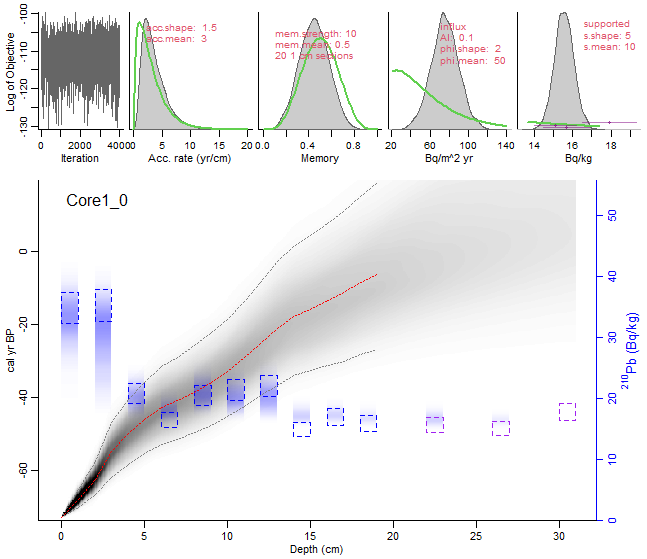
\includegraphics{c01_rplumplot_accmean3.png}
\caption{Core 1 rPlum model run}
\end{figure}

\begin{figure}
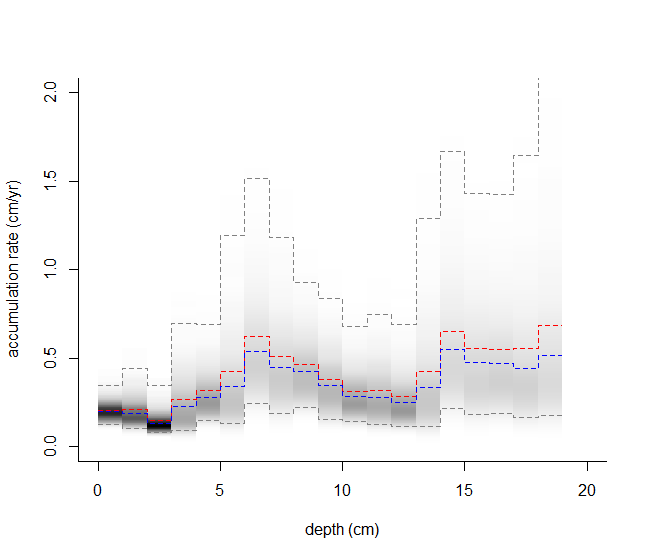
\includegraphics[width=0.5\linewidth]{c01_accdepth_accmean3} 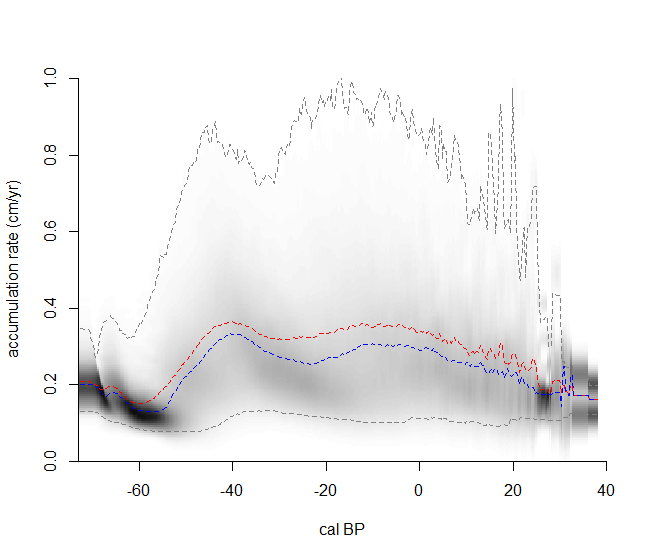
\includegraphics[width=0.5\linewidth]{c01_accage_accmean3} \caption{Accretion by age and depth}\label{fig:agedepth1}
\end{figure}

The age estimate of the core was between 26-45 years at 19 cm (see
Figure 5). On the top layer, sediments accumulate at 0.21 cm/yr. Higher
accumulation rates were found at deeper part of the core. For example,
at 19 cm deep, the accumulation rate was 1.2 cm/yr. This corresponds to
-6 cal BP or 1956 CE. After -50 BP (2000 CE) the accumulation rate
drastically decrease.

\begin{enumerate}
\def\labelenumi{\arabic{enumi}.}
\setcounter{enumi}{1}
\tightlist
\item
  Lead 210 results from Core 4: Healthy eelgrass site The results are
  summarized in Table 4.
\end{enumerate}

\begin{longtable}[]{@{}
  >{\raggedright\arraybackslash}p{(\columnwidth - 10\tabcolsep) * \real{0.1370}}
  >{\raggedleft\arraybackslash}p{(\columnwidth - 10\tabcolsep) * \real{0.1370}}
  >{\raggedleft\arraybackslash}p{(\columnwidth - 10\tabcolsep) * \real{0.2192}}
  >{\raggedleft\arraybackslash}p{(\columnwidth - 10\tabcolsep) * \real{0.1781}}
  >{\raggedleft\arraybackslash}p{(\columnwidth - 10\tabcolsep) * \real{0.1370}}
  >{\raggedleft\arraybackslash}p{(\columnwidth - 10\tabcolsep) * \real{0.1918}}@{}}
\caption{C02: Core data from healthy eelgrass site}\tabularnewline
\toprule\noalign{}
\begin{minipage}[b]{\linewidth}\raggedright
labID
\end{minipage} & \begin{minipage}[b]{\linewidth}\raggedleft
depth(cm)
\end{minipage} & \begin{minipage}[b]{\linewidth}\raggedleft
density(g/cm\^{}3)
\end{minipage} & \begin{minipage}[b]{\linewidth}\raggedleft
210Pb(Bq/kg)
\end{minipage} & \begin{minipage}[b]{\linewidth}\raggedleft
sd(Pb210)
\end{minipage} & \begin{minipage}[b]{\linewidth}\raggedleft
Thickness(cm)
\end{minipage} \\
\midrule\noalign{}
\endfirsthead
\toprule\noalign{}
\begin{minipage}[b]{\linewidth}\raggedright
labID
\end{minipage} & \begin{minipage}[b]{\linewidth}\raggedleft
depth(cm)
\end{minipage} & \begin{minipage}[b]{\linewidth}\raggedleft
density(g/cm\^{}3)
\end{minipage} & \begin{minipage}[b]{\linewidth}\raggedleft
210Pb(Bq/kg)
\end{minipage} & \begin{minipage}[b]{\linewidth}\raggedleft
sd(Pb210)
\end{minipage} & \begin{minipage}[b]{\linewidth}\raggedleft
Thickness(cm)
\end{minipage} \\
\midrule\noalign{}
\endhead
\bottomrule\noalign{}
\endlastfoot
CO4 0\_1 & 1 & 2.19275 & 30.03966 & 2.1521805 & 1 \\
CO4 2\_3 & 3 & 1.14235 & 30.48174 & 2.3924505 & 1 \\
CO4 4\_5 & 5 & 1.58035 & 21.11140 & 1.6877293 & 1 \\
CO4 6\_7 & 7 & 1.21140 & 15.33731 & 1.2817977 & 1 \\
CO4 8\_9 & 9 & 1.48650 & 12.75540 & 1.0901873 & 1 \\
CO4 10\_11 & 11 & 2.08025 & 13.03520 & 1.0943914 & 1 \\
CO4 12\_13 & 13 & 2.40015 & 11.66226 & 1.0354082 & 1 \\
CO4 14\_15 & 15 & 2.97490 & 11.14904 & 0.9963304 & 1 \\
CO4 16\_17 & 17 & 2.89825 & 10.35298 & 0.9441335 & 1 \\
CO4 18\_19 & 19 & 3.09120 & 9.80774 & 0.8979469 & 1 \\
CO4 22\_23 & 23 & 2.95370 & 14.01140 & 1.2506031 & 1 \\
CO4 26\_27 & 27 & 3.15830 & 13.60083 & 1.1953914 & 1 \\
CO4 30\_31 & 31 & 3.00145 & 11.96664 & 1.1005334 & 1 \\
\end{longtable}

The rPlum model was initiated using Pb210 values of the deepest sections
of the core of the as background values. No supplementary radiocarbon
data was used. Figure 4 shows the result of the best fitted with the
following parameters:

\begin{itemize}
\tightlist
\item
  accretion mean: 3
\item
  accretion shape: 1.5
\item
  memory mean: 0.5
\end{itemize}

The age estimate of the core was between 27-44 years at 17 cm (see
Figure xx). On the top layer, sediments accumulate at 0.17 cm/yr. Higher
accumulation rates were found at deeper part of the core. For example,
at 15 cm deep, the accumulation rate was 1.4 cm/yr. This corresponds to
-12 cal BP or 1962 CE. There was a drastic decrease in accretion rate
after cal BP -40 (i.e., 1990 CE) to 0.2 cm/yr and has been decreasing
since then.

\begin{figure}
\centering
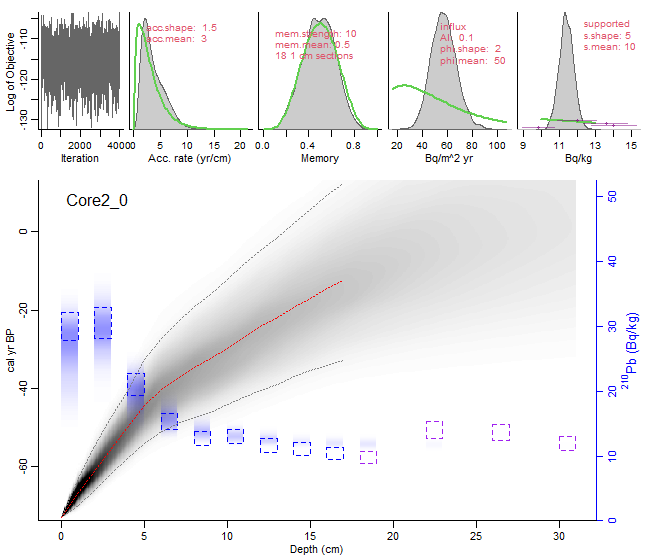
\includegraphics{core2_rplumplot_accmean_3.png}
\caption{Core 2 rPlum model run}
\end{figure}

\begin{figure}
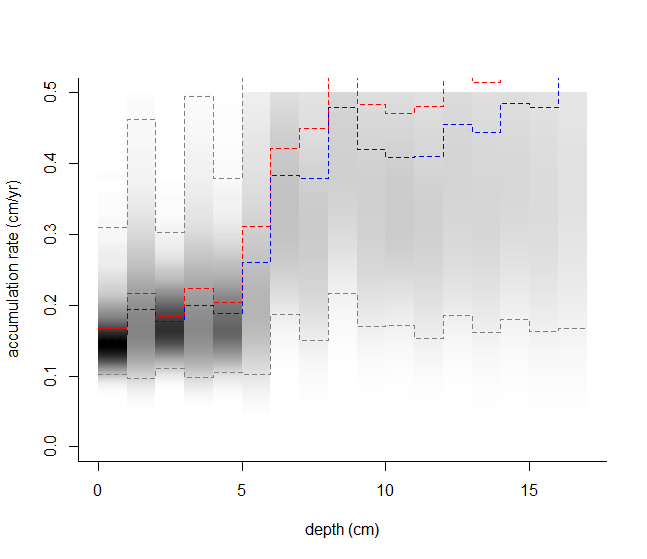
\includegraphics[width=0.5\linewidth]{c02_accdepth_accmean3} 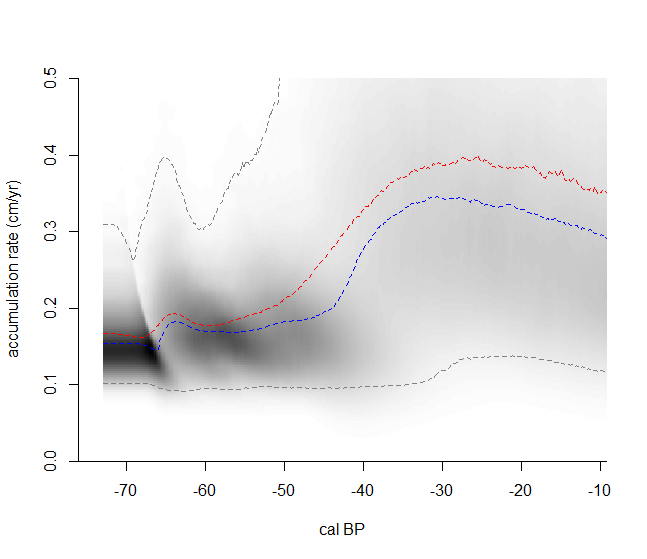
\includegraphics[width=0.5\linewidth]{c02_accage_accmean3} \caption{Accretion by age and depth}\label{fig:agedepth2}
\end{figure}

\newpage

\hypertarget{discussion}{%
\section{Discussion}\label{discussion}}

\begin{enumerate}
\def\labelenumi{\arabic{enumi}.}
\tightlist
\item
  How much organic carbon (C) is James Bay blue carbon ecosystems
  accumulating per unit area? Based on our calculation, the average soil
  organic carbon density of the two sites was approximately 0.02055
  g/cm\textsuperscript{3}, which translates to 20.55
  kg/m\textsuperscript{3}. At this density
\end{enumerate}

\textbf{Carbon Sequestered in 1 square kilometer of eelgrass Soil}

Based on the previous calculation, the average soil organic carbon
density of the two sites was approximately 0.02055 g/cm³, which
translates to 20.55 kg/m³ when converted to kilograms per cubic meter
(kg/m³).

\textbf{Carbon Sequestered in 1 Square Kilometer of Eelgrass Soil:}

Given that the volume of soil in 1 square kilometer area with 1 meter
thickness =
\(1,000,000 \, \text{m}^2 \times 1 \, \text{m} = 1,000,000 \, \text{m}^3\).
The amount of carbon sequestered = Volume of soil \(\times\) Average
soil carbon density =
\(1,000,000 \, \text{m}^3 \times 20.55 \, \text{kg/m}^3 = 20,550,000 \, \text{kg}\)
of carbon.

\textbf{Equivalent Motor Vehicle Emissions:}

Assuming 1 kg of soil organic carbon sequesters about 3.67 kg of CO2
(based on the molecular weight ratio of CO2 to C), the total CO2
sequestered would be
\(20,550,000 \, \text{kg} \times 3.67 = 75,417,350 \, \text{kg of CO2}\).
Converting kilograms to metric tons (since 1 metric ton = 1,000 kg), we
get
\(75,417,350 \, \text{kg} / 1,000 = 75,417.35 \, \text{metric tons of CO2}\).
And given that an average passenger vehicle emits about 4.6 metric tons
of CO2 per year, the number of vehicle emissions this amount of CO2
sequestration represents is
\(75,417.35 \, \text{metric tons CO2} / 4.6 \, \text{metric tons CO2/vehicle/year} \approx 16,393.77 \, \text{vehicles/year}\).
Therefore, a square kilometer of eelgrass soil with 1 meter thickness,
having the average soil carbon density observed in the two sites, can
sequester approximately 75,417.35 metric tons of CO2. This is equivalent
to the annual emissions from approximately 16,394 motor vehicles.

\begin{enumerate}
\def\labelenumi{\arabic{enumi}.}
\setcounter{enumi}{1}
\tightlist
\item
  What are the threats to blue carbon ecosystems, and how do these
  threats affect the sequestration rate of blue carbon in James Bay and
  their traditional ecosystem services?
\end{enumerate}

Eelgrass in James Bay are threatened by development in inland watershed.
The most significant of these development is the contruction and
operation of hydro-electric complex in the region. When the dams were
built,some of the major rivers

\begin{enumerate}
\def\labelenumi{\arabic{enumi}.}
\setcounter{enumi}{2}
\item
  What is the state of James Bay eelgrass and other coastal ecosystems
  as blue carbon sinks/sources? At present, the eelgrass in James Bay is
  a marginal carbon sink. Since the 1990s they are not building their
  sediment as fast as historic rates. If these rate continues and the
  eelgrass fails to recover, eelgrass beds in Chisasibi with be a net
  carbon source.
\item
  How does climate change impact blue carbon accumulation in James Bay?
  Climate change may enhance the capacity eelgrass to absorb more
  carbon, but in the presence of disturbance such as altered hydrology,
  they may become carbon sources. Other ecosystem such as marshes and
  peatlands may expand with rising global temperature which can
  significantly offset regional emissions, however the presence of land
  development such as hydro and mining can reduce extent of peatlands
  and marshes and may cause further methane emission.
\item
  What management actions best maintain and promote carbon sequestration
  and traditional use of blue carbon ecosystems in James Bay?
\end{enumerate}

Improving the state of eelgrass beds by restoration can help bring back
the historical extent of eelgrass beds. However, with constant stressors
such as altered hydrology from damming of rivers, it is unlikely that
sediment accretion rates would improve. It would be more successful if
eelgrass in other areas not affected by La Grande complex can be
restored or enhance.

\begin{itemize}
\tightlist
\item
  Understanding the roles and impacts of toxic cyanobacteria in James
  Bay is beyond the scope of this study, but it is an emerging field of
  research at CERRI.
\end{itemize}

\hypertarget{conlcussion}{%
\section{Conlcussion}\label{conlcussion}}

\begin{itemize}
\item
  There is to some extent a detectable portion of organic sediments
  coming from inland that is being deposited on eelgrass beds. Further
  research is needed to determine whether these organic matter is coming
  from a single river or from multiple rivers.
\item
  Sediments in both healthy and marginal eelgrass beds are becoming more
  sandy with less organic matter and accumulate less and less through
  time.
\end{itemize}

\newpage

\hypertarget{expenses}{%
\section{Expenses}\label{expenses}}

\newpage

\hypertarget{references}{%
\section*{References}\label{references}}
\addcontentsline{toc}{section}{References}

\hypertarget{refs}{}
\begin{CSLReferences}{1}{0}
\leavevmode\vadjust pre{\hypertarget{ref-aquino2018bayesian}{}}%
Aquino-López, Marco A, Maarten Blaauw, J Andrés Christen, and Nicole K
Sanderson. 2018. {``Bayesian Analysis of 210 Pb Dating.''} \emph{Journal
of Agricultural, Biological and Environmental Statistics} 23 (3):
317--33.

\leavevmode\vadjust pre{\hypertarget{ref-howard2014coastal}{}}%
Howard, J, S Hoyt, K Isensee, M Telszewski, and E Pidgeon. 2014.
{``Coastal Blue Carbon: Methods for Assessing Carbon Stocks and
Emissions Factors in Mangroves, Tidal Salt Marshes, and Seagrasses.''}

\leavevmode\vadjust pre{\hypertarget{ref-mathieson2010floristic}{}}%
Mathieson, Arthur C, Gregg E Moore, and Frederick T Short. 2010. {``A
Floristic Comparison of Seaweeds from James Bay and Three Contiguous
Northeastern Canadian Arctic Sites.''} \emph{Rhodora} 112 (952):
396--434.

\end{CSLReferences}

\end{document}
